\documentclass[compress]{beamer}
\usepackage{beamerthemeproyxetex}


%\useoutertheme[footline=authorinstitutetitle]{miniframes}
%\usecolortheme{whale}
%\usecolortheme{orchid}
%\useinnertheme{rounded}


\title{PyNLPl: Python Natural Language Processing Library}
\author{Maarten van Gompel}
\date{05-07-2011}
\usepackage{graphicx}
\usepackage{listings}
\usepackage{color}
\lstset{% general command to set parameter(s)
basicstyle=\footnotesize,
keywordstyle=\color{black}\bfseries,
identifierstyle=\color{blue}\emph,
stringstyle=\color{magenta}\ttfamily,
breaklines=true,
numbers=left,
numberstyle=\footnotesize,
}


\begin{document}

\begin{frame}
	\titlepage\smallraccoon\ilkuvt
\end{frame}

\section{Introduction}

\begin{frame}{First things first}

    \textbf{PyNLPL} is pronounced as...
    \begin{center}
    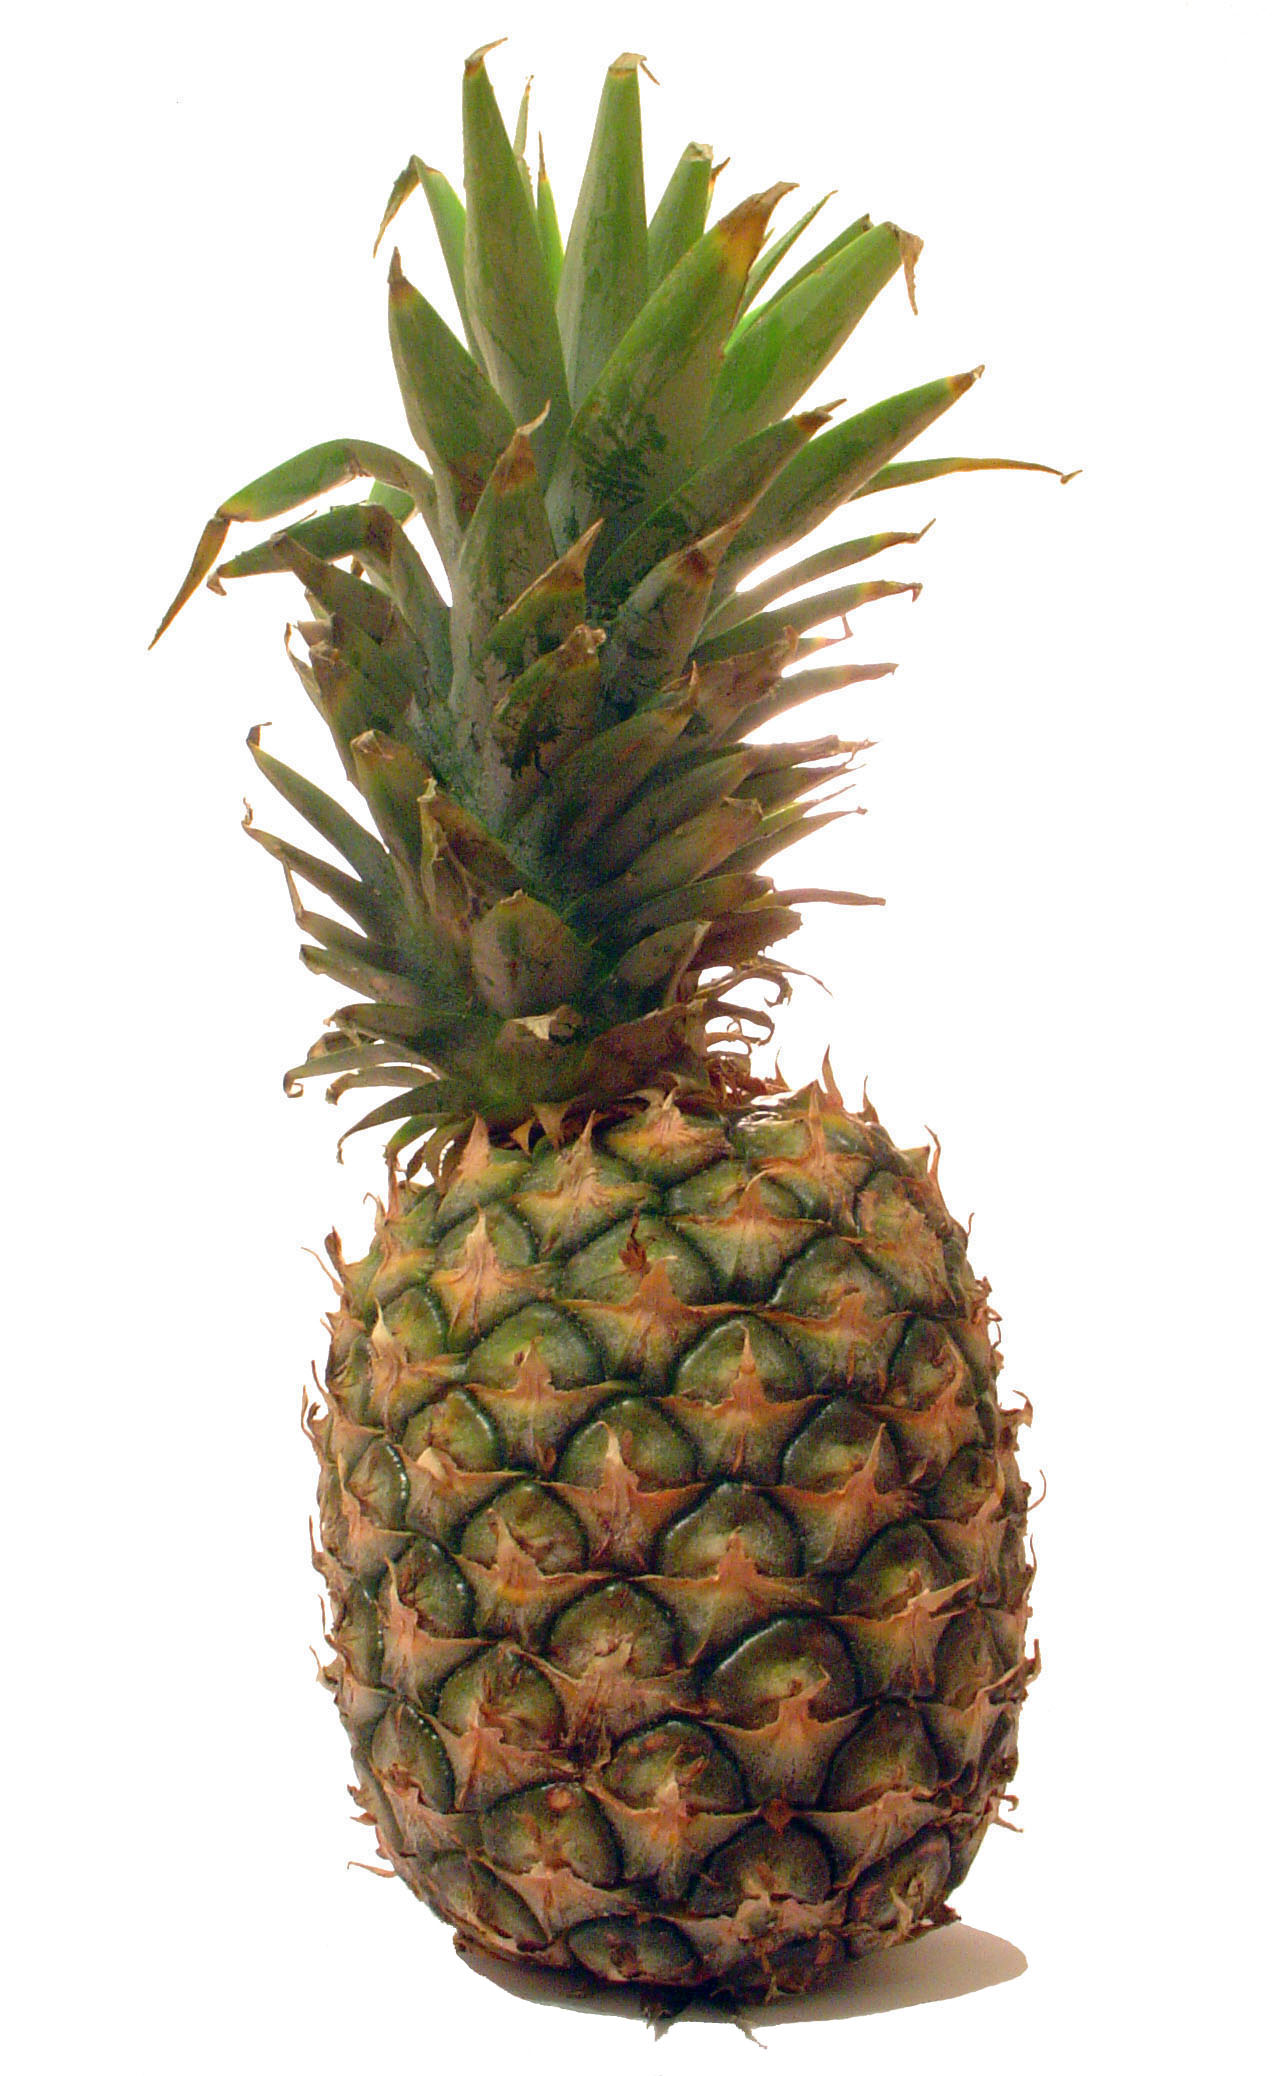
\includegraphics[width=40.0mm]{pineapple.jpg}
    \end{center}

\end{frame}

\begin{frame}{Introduction}


    \begin{block}{What is PyNLPl?}
        \textbf{Python Natural Language Processing Library}
        
        
        
        \begin{itemize}
            \item A collection of custom-made Python modules usable in Natural Language Processing
            \item Very modular setup
            \item Reusable object-oriented modules, prevents ``reinventing the wheel'' for common tasks
            \item Using PyNLPl enables you to more quickly write NLP tools, as you need not start from scratch.
        \end{itemize}
        

    \end{block}

\end{frame}

\subsection{Installation}

\begin{frame}{Installation}

    \begin{block}{Installation}
        PyNLPl is on github:        
        \texttt{http://github.com/proycon/pynlpl}
        
        To obtain it: 
        \texttt{\$ git clone https://github.com/proycon/pynlpl}
        
        And for ILK, it's also in our private SVN:
        \texttt{\$ svn checkout https://ilk.uvt.nl/svn/trunk/sources/pynlpl/}
    \end{block}

\end{frame}

\subsection{Q \& A}

\begin{frame}{Questions and Answers (1/4)}

        \textbf{Q:} Why reinvent the wheel yourself and not use for example NLTK? \\
        \textbf{A:} Firstly because there are many customised modules not present in NLTK, such as modules for dealing with FoLiA, D-Coi, Timbl, Cornetto, DutchSemCor. Secondly, because reimplementing things myself was a good learning process to better understand certain algorithms.
\end{frame}


\begin{frame}{Questions and Answers (2/4)}
        
        \textbf{Q:} How did PyNLPl came to be? \\
        \textbf{A:} Often code is (and should be) modular and reusable in the future. Whenever that is the case, I put it into PyNLPl.
\end{frame}

\begin{frame}{Questions and Answers (3/4)}
        
        \textbf{Q:} Where is PyNLPl used? \\
        \textbf{A:} In almost everything I write: PBMBMT, Valkuil, the DutchSemCor Supervised-WSD system heavily rely on PyNLPl.
\end{frame}
        
\begin{frame}{Questions and Answers (4/4)}

        \textbf{Q:} Why Python? \\
        \textbf{A:} Elegant, modern and powerful scripting language, short development time. Great for text processing, easy to learn. Substantial user-base and 3rd party libraries available.        
\end{frame}

\section{Contents}

\begin{frame}{Packages and modules in PyNLPl (1/3)}
    \begin{block}{Packages and modules in PyNLPl (1/3)}
        \begin{itemize}
            \item \texttt{pynlpl.statistics} -- Module containing classes and functions for statistics
            \item \texttt{pynlpl.evaluation} -- Module for evaluation and experimentation, such as computation of precision/recall, creation of confusion matrices, etc.. Also contains abstract experiment classes and Wrapped Progressive Sampling.
            \item \texttt{pynlpl.datatypes} -- Module containing data types
            \item \texttt{pynlpl.search} -- Module containing search algorithms
            \item \texttt{pynlpl.textprocessors} -- Module containing text processors
        \end{itemize}
    \end{block}

\end{frame}

\begin{frame}{Packages and modules in PyNLPl (2/3)}
    \begin{block}{Packages and modules in PyNLPl (2/3)}
        \begin{itemize}
            \item \texttt{pynlpl.formats} -- Contains modules for reading/writing specific file formats
            \begin{itemize}
                \item \texttt{pynlpl.formats.timbl} -- Module for reading Timbl output format
                \item \texttt{pynlpl.formats.sonar} -- Module for reading the SoNaR corpus (D-Coi XML)
                \item \texttt{pynlpl.formats.folia} - Module for reading/writing FoLiA XML
                \item \texttt{pynlpl.formats.giza} - Module containing class for reading giza A3 alignment
                \item \texttt{pynlpl.formats.moses} - Module containing class for reading phrase translation tabel                
                \item \texttt{pynlpl.formats.cgn} -- \texttt{pynlpl.formats.dutchsemcor}
            \end{itemize}
        \end{itemize}
    \end{block}

\end{frame}
    
\begin{frame}
    \begin{block}{Packages and modules in PyNLPl (3/3)}
        \begin{itemize}
            \item \texttt{pynlpl.clients} -- Contains network clients for various services.
            \begin{itemize}
                \item \texttt{pynlpl.clients.cornetto} -- Client to connect to Cornetto webservice
                \item \texttt{pynlpl.clients.frogclient} -- Client to connect to Frog server
            \end{itemize}
            \item \texttt{pynlpl.lm} -- Language Models
            \begin{itemize}
                \item \texttt{pynlpl.lm.lm} -- Contains simple language model
                \item \texttt{pynlpl.lm.srilm} -- SRILM module
                \item \texttt{pynlpl.lm.server} -- Generic LM Server
            \end{itemize}
        \end{itemize}
    \end{block}

\end{frame}
    
\section{Code Samples}    
    
\begin{frame}[fragile]
\textbf{Using pynlpl.statistics: FrequencyList and Distribution}

\begin{lstlisting}[language=python]
>>> from pynlpl.statistics import FrequencyList, Distribution
>>> freqlist = FrequencyList()
>>> freqlist.append(['It','is','what','is','is'])
>>> freqlist
{'It': 1, 'it': 1, 'is': 2, 'what': 1}
>>> freqlist['is']
2
>>> dist = Distribution(freqlist)
>>> dist
{'It': 0.2, 'it': 0.2, 'is': 0.4, 'what': 0.2}
>>> dist['is']
0.4
>>> dist.entropy()
1.9219280948873623
\end{lstlisting}

\end{frame}




\begin{frame}[fragile]

\textbf{Creating N-grams with pynlpl.textprocessors.Windower}

\begin{lstlisting}[language=python]
>>> from pynlpl.textprocessors import Windower
>>> s = ['It','is','what','it','is']
>>> list(Windower(s,2))
[('<begin>', 'It'), ('It', 'is'), ('is', 'what'), 
('what', 'it'), ('it', 'is'), ('is', '<end>')]
\end{lstlisting}


\end{frame}
        



\begin{frame}[fragile]

\textbf{Combining things: Creating a tri-gram frequency list from a FoLiA document} 

\begin{lstlisting}[language=python]
>>> from pynlpl.formats import folia
>>> from pynlpl.statistics import FrequencyList
>>> doc = folia.Document(file='/path/to/folia_doc.xml')
>>> freqlist = FrequencyList()
>>> for trigram in Windower(doc.words(),3,False,False):
...       freqlist.count(trigram)
>>> freqlist.save('freqlist.txt')
\end{lstlisting}

\end{frame}
    

\begin{frame}[fragile]

\textbf{Creating a simple trigram Language Model of a corpus in FoLiA or DCOI XML} 

\begin{lstlisting}[language=python]
>>> from pynlpl.formats.folia import Corpus
>>> from pynlpl.statistics import FrequencyList
>>> simplelm = SimpleLanguageModel(3)
>>> for doc in Corpus('/path/to/for/example/sonar/')
...     for sentence in doc.sentences():
...         simpelm.append([ word.text() for word in sentence.words()])
>>> simplelm.save('sonar.trigram.lm')   
\end{lstlisting}


\end{frame}


\begin{frame}[fragile]

\textbf{Using the Frog Client}

First start Frog in server mode: \verb|frog --skip=p -S 12345|

\begin{lstlisting}[language=python]
>>> from pynlpl.clients.frogclient import FrogClient
>>> client = FrogClient('localhost',12345)
>>> for word, lemma, morph, pos in client.process("Het is wat het is"):
...     print lemma, pos
het VNW(pers,pron,stan,red,3,ev,onz)
zijn WW(pv,tgw,ev)	
wat VNW(vb,pron,stan,vol,3o,ev)
het VNW(pers,pron,stan,red,3,ev,onz)
zijn WW(pv,tgw,ev)
\end{lstlisting}

\end{frame}

\begin{frame}[fragile]

\textbf{Using the evaluation module (1/2)} 

\footnotesize
\begin{lstlisting}[language=python]
>>> from pynlpl.evaluation import ClassEvaluation
>>> weather_forecast = ['sun','sun','rain','cloudy']
>>> actual_weather = ['cloudy','sun','rain','rain']
>>> evl = ClassEvaluation(actual_weather, weather_forecast)
>>> print evl
                TP	FP	TN	FN	Accuracy	Precision	Recall(TPR)	Specificity(TNR)	F-score
sun             1	1	2	0	0.750000	0.500000	1.000000	0.666667	0.666667
cloudy          0	1	2	1	0.500000	0.000000	0.000000	0.666667	 nan
rain            1	0	2	1	0.750000	1.000000	0.500000	1.000000	0.666667

Accuracy             : 0.5
Recall      (macroav): 0.625
Precision   (macroav): 0.5
Specificity (macroav): 0.75
F-score     (macroav): nan
>>> evl.accuracy()
0.5
>> evl.accuracy('sun')
0.75
\end{lstlisting}
\normalsize


\end{frame}

\begin{frame}[fragile]
 
\textbf{Using the evaluation module (2/2)} 

\begin{lstlisting}[language=python]
>>> evl.confusionmatrix()
{('cloudy', 'sun'): 1, ('rain', 'cloudy'): 1, ('sun', 'sun'): 1, ('rain', 'rain'): 1}
>> print evl.confusionmatrix()
== Confusion Matrix == (hor: goals, vert: observations)

                     cloudy rain  sun
              cloudy      0    1    0
                rain      0    1    0
                 sun      1    0    1
\end{lstlisting}


\end{frame}

\section{Complex topics}

\begin{frame}{Complex topics}

\begin{block}{Search Algorithms} 
\begin{enumerate}
 \item Define your search state, a class derived from the abstract class \texttt{pynlpl.search.AbstractSearchState}
 \item Add methods \texttt{expand()} and for informed searches \texttt{score()}
 \item Instantiate an initial search state
 \item Pass this to the search algorithm of your choice, there are several implemented in \texttt{pynlpl.search}: DepthFirstSearch, BreadthFirstSearch, IterativeDeepening, BestFirstSearch, BeamSearch, HillClimbingSearch, StochasticBeamSearch
 \item Obtain the solution(s) and/or path(s)
\end{enumerate}
\end{block}


\end{frame}


\begin{frame}{Experiments}

\begin{block}{Experiments} 

You can define your experiment, as a class derived from the abstract class \texttt{pynlpl.evaluation.AbstractExperiment}. Overloading methods as \texttt{run()}, \texttt{start()} \\


You can then use these with \texttt{pynlpl.evaluation.ExperimentPool} for multi-threaded use and in \texttt{pynlpl.evaluation.ParamSearch} and \texttt{pynlpl.evaluation.WPSParamSearch} for parameter optimisation.

\end{block}

\end{frame}

\section{Conclusion}

\begin{frame}{Conclusion}

    \begin{block}{Contribute!}
        If you have a modular, re-usable, preferably object-oriented Python module useful for NLP tasks. Consider adding it to PyNLPl!                    
    \end{block}

 \begin{block}{Conclusion (shameless promotion)}
    \begin{itemize}
    \item \textbf{Use} PyNLPl if it has modules you can use!
    \item \textbf{Contribute} to PyNLPl with new modules!
    \end{itemize}
    
 \end{block}
 
 \smallraccoon
\end{frame}


    


\end{document}
